\chapter{Data and Simulated Samples}
The data sample used for the \hzg search corresponds to a total integrated luminosity of \LumiT\fbinv and was collected over a data-taking period spanning three years: \Lumia\fbinv in 2016, \Lumib\fbinv in 2017, and \Lumic\fbinv in 2018~\cite{CMS-LUM-17-003,LUM-17-004,LUM-18-002}. 
To be considered in the analysis, events must satisfy the high-level trigger requirements for at least one of the dielectron or dimuon triggers.
The dielectron trigger requires a leading (subleading) electron with
$\pt > 23\,(12)\GeV$, while the dimuon trigger requires a muon with $\pt > 17\,(8)\GeV$.
The corresponding CMS data streams are listed in Table \ref{tab:data_samples}. To ensure data quality, luminosity masks are applied based recommendations from the Physics Performance and Dataset group. Table \ref{tab:lumi_jsons} shows the luminosity masks applied for each of the three data-taking years.

\begin{table}[h]
  \begin{center}
    \caption{Summary of data samples used.}
    \begin{tabular}{|l|l|}
      \hline
      data set name                                    & channel                       \\ \hline
      /DoubleEG/Run2016B-17Jul2018\_ver2-v1/MINIAOD   & $\PZ\PGg\to \Pe\Pe + \PGg $     \\
      /DoubleEG/Run2016C-17Jul2018-v1/MINIAOD         & $\PZ\PGg\to \Pe\Pe + \PGg $     \\
      /DoubleEG/Run2016D-17Jul2018-v1/MINIAOD         & $\PZ\PGg\to \Pe\Pe + \PGg $     \\
      /DoubleEG/Run2016E-17Jul2018-v1/MINIAOD         & $\PZ\PGg\to \Pe\Pe + \PGg $     \\       
      /DoubleEG/Run2016F-17Jul2018-v1/MINIAOD         & $\PZ\PGg\to \Pe\Pe + \PGg $     \\       
      /DoubleEG/Run2016G-17Jul2018-v1/MINIAOD         & $\PZ\PGg\to \Pe\Pe + \PGg $     \\
      /DoubleEG/Run2016H-17Jul2018-v1/MINIAOD         & $\PZ\PGg\to \Pe\Pe + \PGg $     \\
      /DoubleEG/Run2016H-17Jul2018-v1/MINIAOD         & $\PZ\PGg\to \Pe\Pe + \PGg $     \\
      /DoubleEG/Run2017B-31Mar2018-v1/MINIAOD         & $\PZ\PGg\to \Pe\Pe + \PGg $     \\
      /DoubleEG/Run2017C-31Mar2018-v1/MINIAOD         & $\PZ\PGg\to \Pe\Pe + \PGg $     \\
      /DoubleEG/Run2017D-31Mar2018-v1/MINIAOD         & $\PZ\PGg\to \Pe\Pe + \PGg $     \\
      /DoubleEG/Run2017E-31Mar2018-v1/MINIAOD         & $\PZ\PGg\to \Pe\Pe + \PGg $     \\       
      /DoubleEG/Run2017F-31Mar2018-v1/MINIAOD         & $\PZ\PGg\to \Pe\Pe + \PGg $     \\           
      /EGamma/Run2018A-17Sep2018-v2/MINIAOD           & $\PZ\PGg\to \Pe\Pe + \PGg $     \\  
      /EGamma/Run2018B-17Sep2018-v1/MINIAOD           & $\PZ\PGg\to \Pe\Pe + \PGg $     \\
      /EGamma/Run2018C-17Sep2018-v1/MINIAOD           & $\PZ\PGg\to \Pe\Pe + \PGg $     \\
      /EGamma/Run2018D-22Jan2019-v2/MINIAOD           & $\PZ\PGg\to \Pe\Pe + \PGg $     \\
      \hline  
      \hline  
      /DoubleMuon/Run2016B-17Jul2018\_ver2-v1/MINIAOD   & $\PZ\PGg\to \PGm\PGm + \PGg $     \\
      /DoubleMuon/Run2016C-17Jul2018-v1/MINIAOD         & $\PZ\PGg\to \PGm\PGm + \PGg $     \\
      /DoubleMuon/Run2016D-17Jul2018-v1/MINIAOD         & $\PZ\PGg\to \PGm\PGm + \PGg $     \\
      /DoubleMuon/Run2016E-17Jul2018-v1/MINIAOD         & $\PZ\PGg\to \PGm\PGm + \PGg $     \\
      /DoubleMuon/Run2016F-17Jul2018-v1/MINIAOD         & $\PZ\PGg\to \PGm\PGm + \PGg $     \\
      /DoubleMuon/Run2016G-17Jul2018-v1/MINIAOD         & $\PZ\PGg\to \PGm\PGm + \PGg $     \\ 
      /DoubleMuon/Run2016H-17Jul2018-v1/MINIAOD         & $\PZ\PGg\to \PGm\PGm + \PGg $     \\
      /DoubleMuon/Run2016H-17Jul2018-v1/MINIAOD         & $\PZ\PGg\to \PGm\PGm + \PGg $     \\ 
      /DoubleMuon/Run2017B-31Mar2018-v1/MINIAOD         & $\PZ\PGg\to \PGm\PGm + \PGg $     \\
      /DoubleMuon/Run2017C-31Mar2018-v1/MINIAOD         & $\PZ\PGg\to \PGm\PGm + \PGg $     \\
      /DoubleMuon/Run2017D-31Mar2018-v1/MINIAOD         & $\PZ\PGg\to \PGm\PGm + \PGg $     \\
      /DoubleMuon/Run2017E-31Mar2018-v1/MINIAOD         & $\PZ\PGg\to \PGm\PGm + \PGg $     \\       
      /DoubleMuon/Run2017F-31Mar2018-v1/MINIAOD         & $\PZ\PGg\to \PGm\PGm + \PGg $     \\
      /DoubleMuon/Run2018A-17Sep2018-v2/MINIAOD         & $\PZ\PGg\to \PGm\PGm + \PGg $     \\  
      /DoubleMuon/Run2018B-17Sep2018-v1/MINIAOD         & $\PZ\PGg\to \PGm\PGm + \PGg $     \\
      /DoubleMuon/Run2018C-17Sep2018-v1/MINIAOD         & $\PZ\PGg\to \PGm\PGm + \PGg $     \\
      /DoubleMuon/Run2018D-PromptReco-v2/MINIAOD        & $\PZ\PGg\to \PGm\PGm + \PGg $     \\\hline       
    \end{tabular}
    \label{tab:data_samples}
  \end{center}
\end{table}

\begin{table}[h]
    \scriptsize
  \begin{center}
    \caption{JSON files for luminosity masks used in the analysis.}
    \begin{tabular}{|l|l|l|}
      \hline
        run period &  JSON file   &     luminosity ($fb^{-1}$)   \\ \hline
        2016       &  Cert\_271036-284044\_13TeV\_ReReco\_07Aug2017\_Collisions16\_JSON.txt   & \Lumia    \\
        2017       &  Cert\_294927-306462\_13TeV\_EOY2017ReReco\_Collisions17\_JSON\_v1.txt   & \Lumib    \\
        2018       &  Cert\_314472-325175\_13TeV\_17SeptEarlyReReco2018ABC\_PromptEraD\_Collisions18\_JSON.txt    & \Lumic    \\
      \hline
    \end{tabular}
    \label{tab:lumi_jsons}
  \end{center}
\end{table}

Signal samples for $\Pg\Pg\PH$, VBF, $\mathrm{V}\PH$, and $\ttbar\PH$ production, with 
$\PH\to\PZ\gamma$ and $\PZ\to\ell^+\ell^-$ ($\ell = \Pe$, $\mu$, or $\tau$),
are generated at next-to-leading order (NLO) using \POWHEG v2.0~\cite{cite:powheg1,cite:powheg2}.
Samples are produced for $m_\PH$ of $120$, $125$, and $130$\GeV. 
The SM Higgs boson production cross sections and branching fractions
recommended by the LHC Higgs Working
Group~\cite{LHC-YR4} are considered for each mass point.

The dominant backgrounds, $\PZ/\gamma^{*}(\rightarrow \ell^+\ell^-)$+$\gamma$ and $\PZ/\gamma^{*}(\rightarrow \ell^+\ell^-)$+jets,
are generated at NLO using the \MGvATNLO v2.6.0 (v2.6.1) 
generator~\cite{Alwall:2014hca} for 2016 (2017 and 2018) samples. 
 Events arising from $\ttbar$ production~\cite{Frixione:2007nw} are a relatively minor background and are generated at NLO with \POWHEG v2.0~\cite{cite:powheg1,cite:powheg2}.
 The background from vector boson scattering (VBS) production of $\PZ/\gamma^{*}$+$\gamma$ pairs, with the $\PZ$ boson decaying to a pair of leptons, is simulated at leading order using the \MGvATNLO generator. The decay $\PH\to\mu^+\mu^-$ is considered as a resonant background and is generated for the $\Pg\Pg\PH$, VBF,  $\mathrm{V}\PH$, and $\ttbar\PH$ production mechanisms. The $\Pg\Pg\PH$ production cross section is
computed at next-to-next-to-NLO precision in QCD and at NLO in electroweak (EWK)
theory~\cite{Anastasiou:2016cez}. 
The cross sections for Higgs boson production in the VBF~\cite{PhysRevLett.115.082002} and VH~\cite{BREIN2004149} mechanisms are calculated at next-to-NLO in QCD, including NLO EWK corrections, while the $\ttbar\PH$ cross section is computed at NLO in QCD and EWK theory~\cite{PhysRevD.68.034022}. 

All simulated events are interfaced
with \PYTHIA v8.226~(v8.230)~\cite{Sjostrand:2014zea} with the
CUETP8M1~\cite{Khachatryan:2015pea} (CP5~\cite{Sirunyan:2019dfx}) underlying event tune for 2016 (2017--2018) for the
fragmentation and hadronization of partons and the internal bremsstrahlung of the leptons. The NLO parton distribution function (PDF) set, NNPDF v3.0~\cite{nnpdf30}~(NNPDF v3.1)~\cite{nnpdf_new}, is used to produce these samples in 2016 (2017--2018). The response of the CMS detector is modeled using the
\GEANTfour  program~\cite{AGOSTINELLI2003250}. 
The simulated events are reweighted to correct for differences between data and simulation in the number of additional $\Pp\Pp$ interactions, trigger efficiencies, selection efficiencies, and efficiencies of isolation requirements for photons, electrons, and muons.

\section{Z+jets Overlap Removal}
In the simulation of the Z+jets sample, PYTHIA adds ISR and FSR photons to the events.
However, these events overlap with those in SM $\PZ\PGg$ sample. 
In addition, the ISR and FSR photons 
in the SM $\PZ\PGg$ sample are simulated at the matrix element level, and the interference between
the ISR and FSR $\PZ\PGg$ diagrams is better computed in Madgraph. 
Therefore the overlapping events are removed from the Z+jets sample 
and retained in the SM $\PZ\PGg$ sample. Events are identified as 
overlapping if they contain at least one photon which is either flagged as 
``fromHardProcessFinalState'' nor ``isPromptFinalState'' with $\Delta R < 0.1$ , $\Delta R = \sqrt{\Delta\eta^2+\Delta\phi^2}$,
with respect to the selected reconstructed photon. 

\section{Photon Internal Conversion}
\label{sec:gconversion}
It was noticed by the $\PH\to\PGg\PGg$ group that Pythia 8 showering automatically 
includes a component in which $\PH\to\PGg\PGg$ photons are 
``internally converted'' into  $\PH\to\PGg\PGg*\to ff\PGg\PGg$ 
(with $ff$ mostly $ee$). This also affects the $\PH\to \PZ\PGg$ and SM $\PZ\PGg$ samples. 
We lose some events with $\PGg^{*}$ decay to fermions since they do not pass our selection of 
2 leptons plus a photon. 
Since the normalization of the samples 
does not include the internal conversion component, the cross section has to be adjusted accordingly.
To determine the number by which the cross section is adjusted, we measure the internal conversion
rate in MC. 
We define a ratio where the numerator is the number of photons flagged as
\textbf{fromHardProcessFinalState} 
and the denominator is total number of events in the MC. Subtracting this ratio from 1 gives
the internal conversion rate.
In our analysis, the internal conversion rate is ~3.1\%(2016) and ~3.0\%(2017).  
We therefore divide our cross sections by 0.969 (0.97) for 2016 (2017 and 2018).

\section{$ll\gamma$ \pt Reweighting}\label{sec:Zpt}
For the 2016 MC, the underlying event tuning was developed in Run-1 with 7 \TeV data. 
To get a more appropriate underlying description, the GEN group provided a new tuning
for 2017 and 2018 MC production, updating from CUETP8M1 (2016) to CP5 (2017/2018).
However, a discrepency was found in the $\ell\ell\gamma$ \pt spectrum
which had an obvious and significant impact in the SM $Z\gamma$ sample. 
Since $\pt^{ll\gamma}/m_{ll\gamma}$ is an important variable in the kinematic MVA training, 
we correct for this issue by reweighting the $\pt^{ll\gamma}$ from simulation to data in 
2017 and 2018 using a sideband region. 
We define the sideband region as $115GeV<m_{ll\gamma}<120GeV$ and $130GeV<m_{ll\gamma}<135GeV$,
which is chosen close to signal region to avoid differences in kinematics.
We evaluate this weight for the electron and muon channels for 2017 and 2018.
\begin{figure*}[htbp]
	\begin{center}
		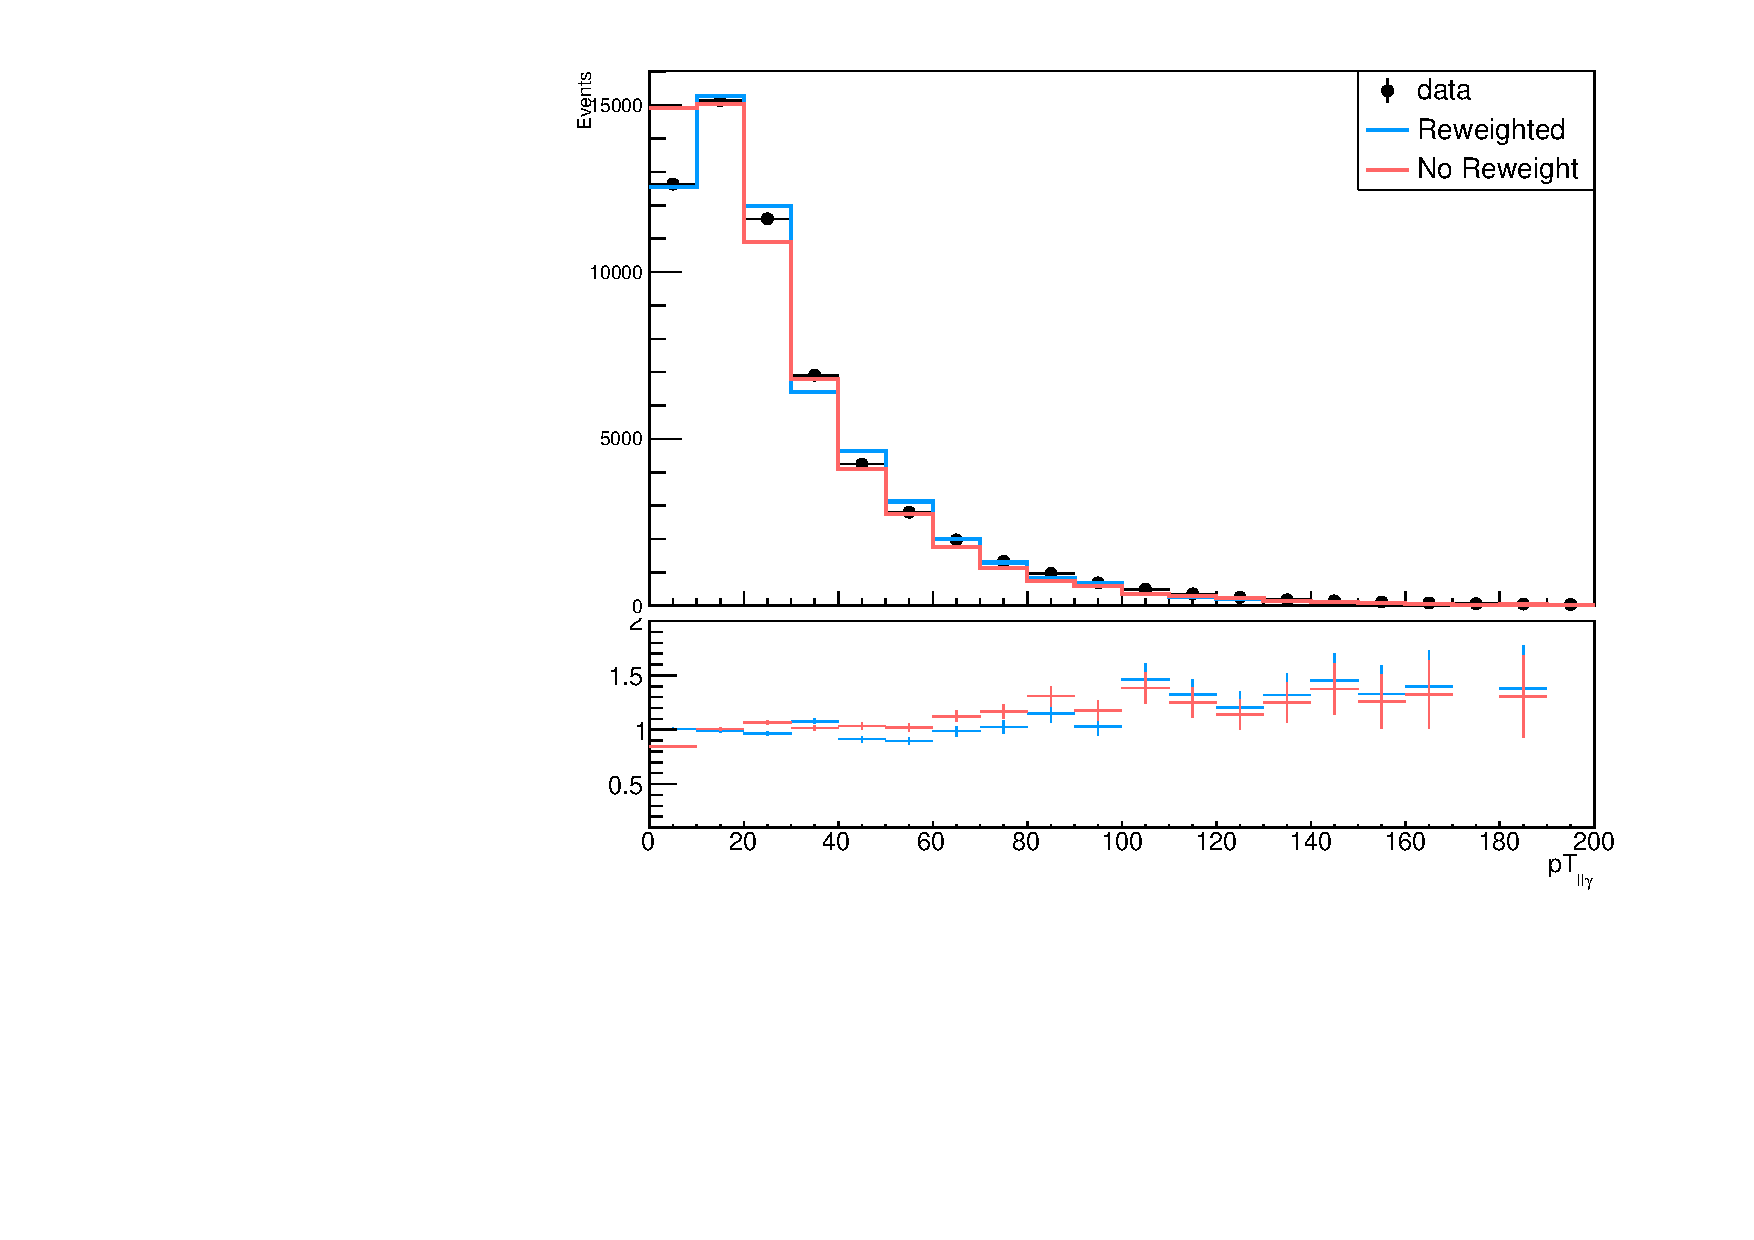
\includegraphics[width=0.35\textwidth]{fig/zpt_reweight/zgptrewei_datasb17.pdf}
		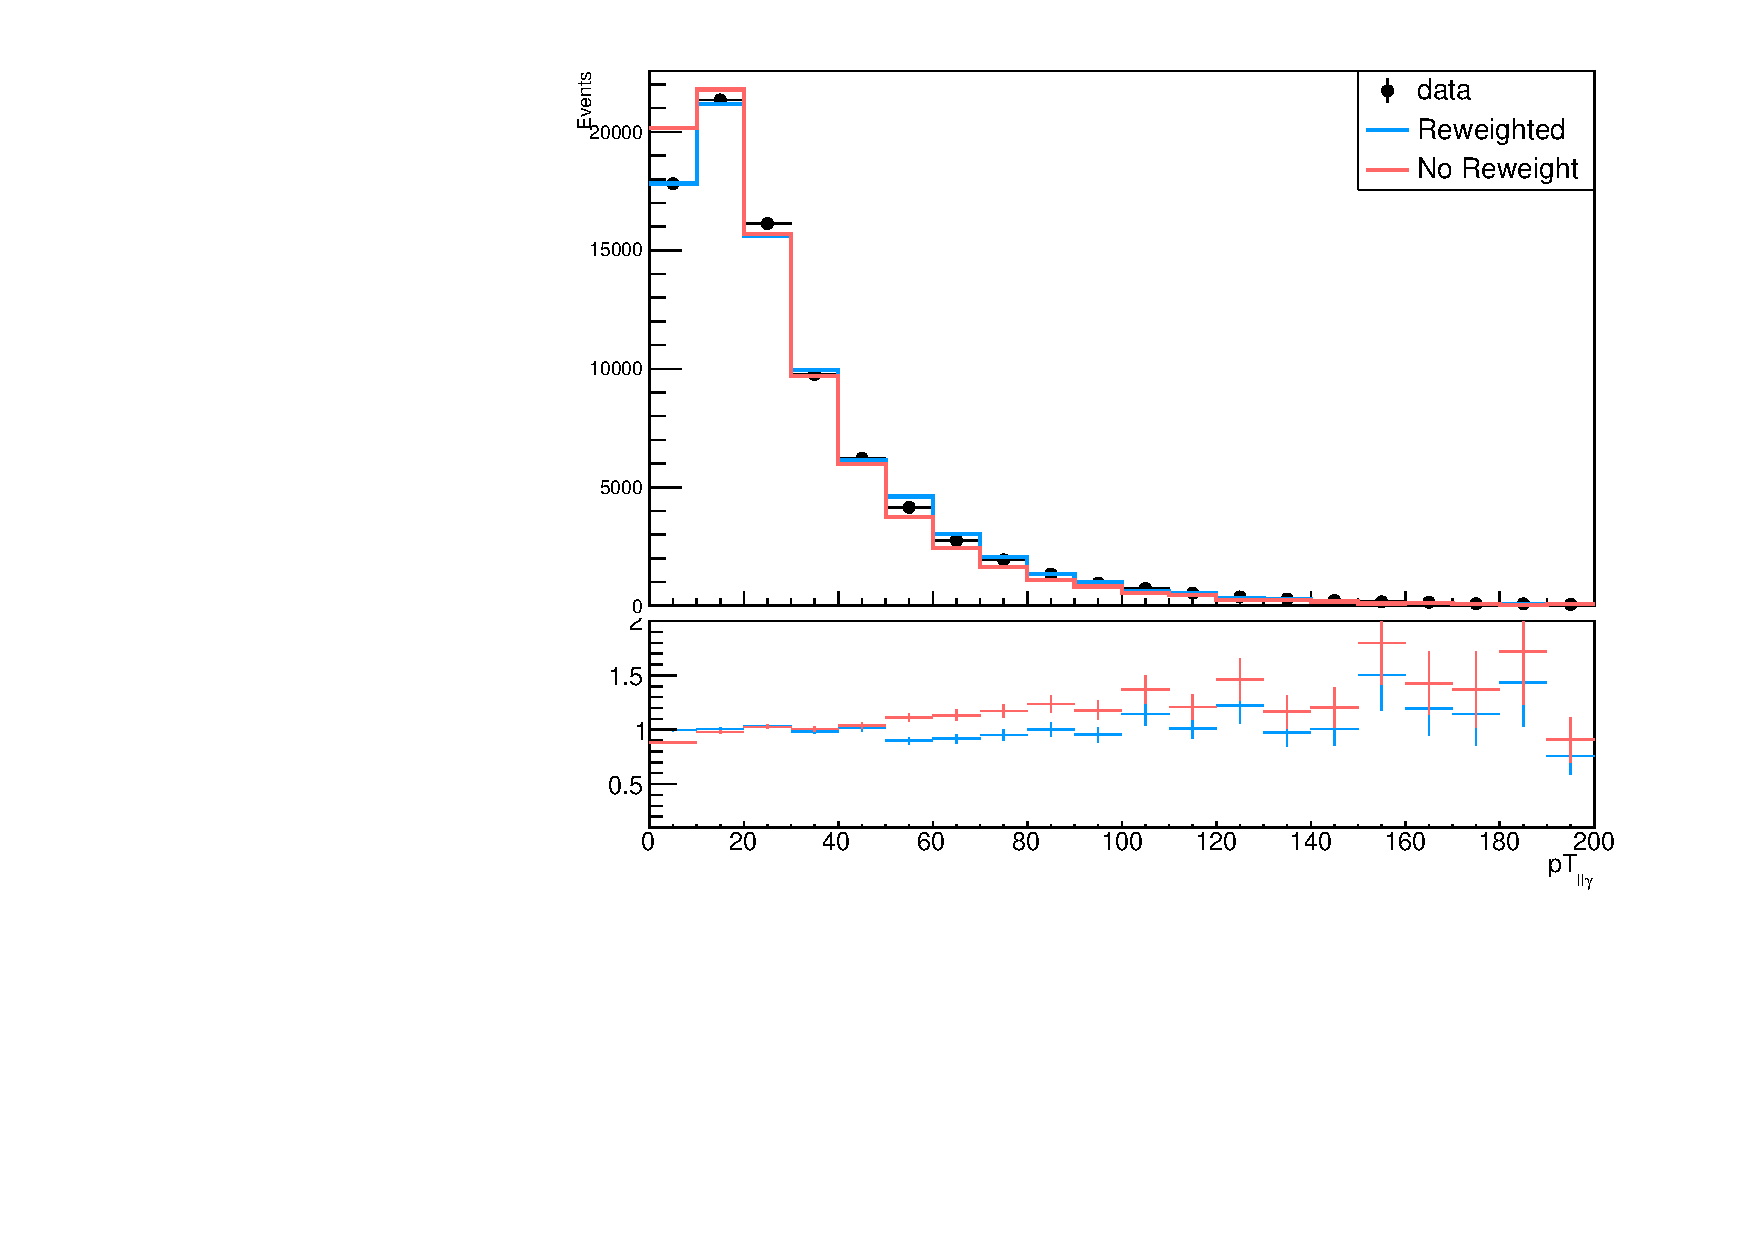
\includegraphics[width=0.35\textwidth]{fig/zpt_reweight/zgptrewei_datasb18.pdf}
	\end{center}
	\caption{Simulation before and after the correction to the $\ell\ell\gamma$ \pt.
    The black points show the data. Left:2017, right: 2018.}
\end{figure*}

\section{Pileup Reweighting}\label{sec:pileup}
The simulation includes an accurate distribution of the number of interactions 
taking place in each bunch crossing. Although the Deterministic Annealing primary vertex reconstruction \cite{detanneal} has been shown to
be efficient and well-behaved up to the observed levels of pileup, the final distribution
for the number of reconstructed primary vertices is still sensitive to differences between data and 
MC in the primary vertex reconstruction and underlying event.
Additionally, there is a potentially larger effect where the distribution for the number of
reconstructed vertices can be biased by the offline event selection criteria and even by the trigger.
In order to factorize these effects, instead of reweighting the MC by the number of 
reconstructed Primary Vertices, we reweight the number of pileup interactions in the simulation 
(as stored in the PileupInfo collection in the MC). The pileup distribution for data is
derived by using the per-bunch-crossing-per-luminosity-section instantaneous luminosity from
the LumiDB together with the total pp inelastic cross section. The total pp inelastic cross 
section is taken to be 66 mb, 72.4 mb, and 80 mb for 2016, 2017, and 2018 respectively.
This yields an expected pileup distribution, correctly weighted by the 
per-bunch-crossing-per-luminosity-section integrated luminosity over the entire data-taking period. The inelatistic cross-sections are choosing the  
Figure \ref{fig:puwei} shows the number of primary vertices distribution after 
pile-up reweighting in
the $ee\PGg$ channel. 
\begin{figure}[hbtp]
  \begin{center}
     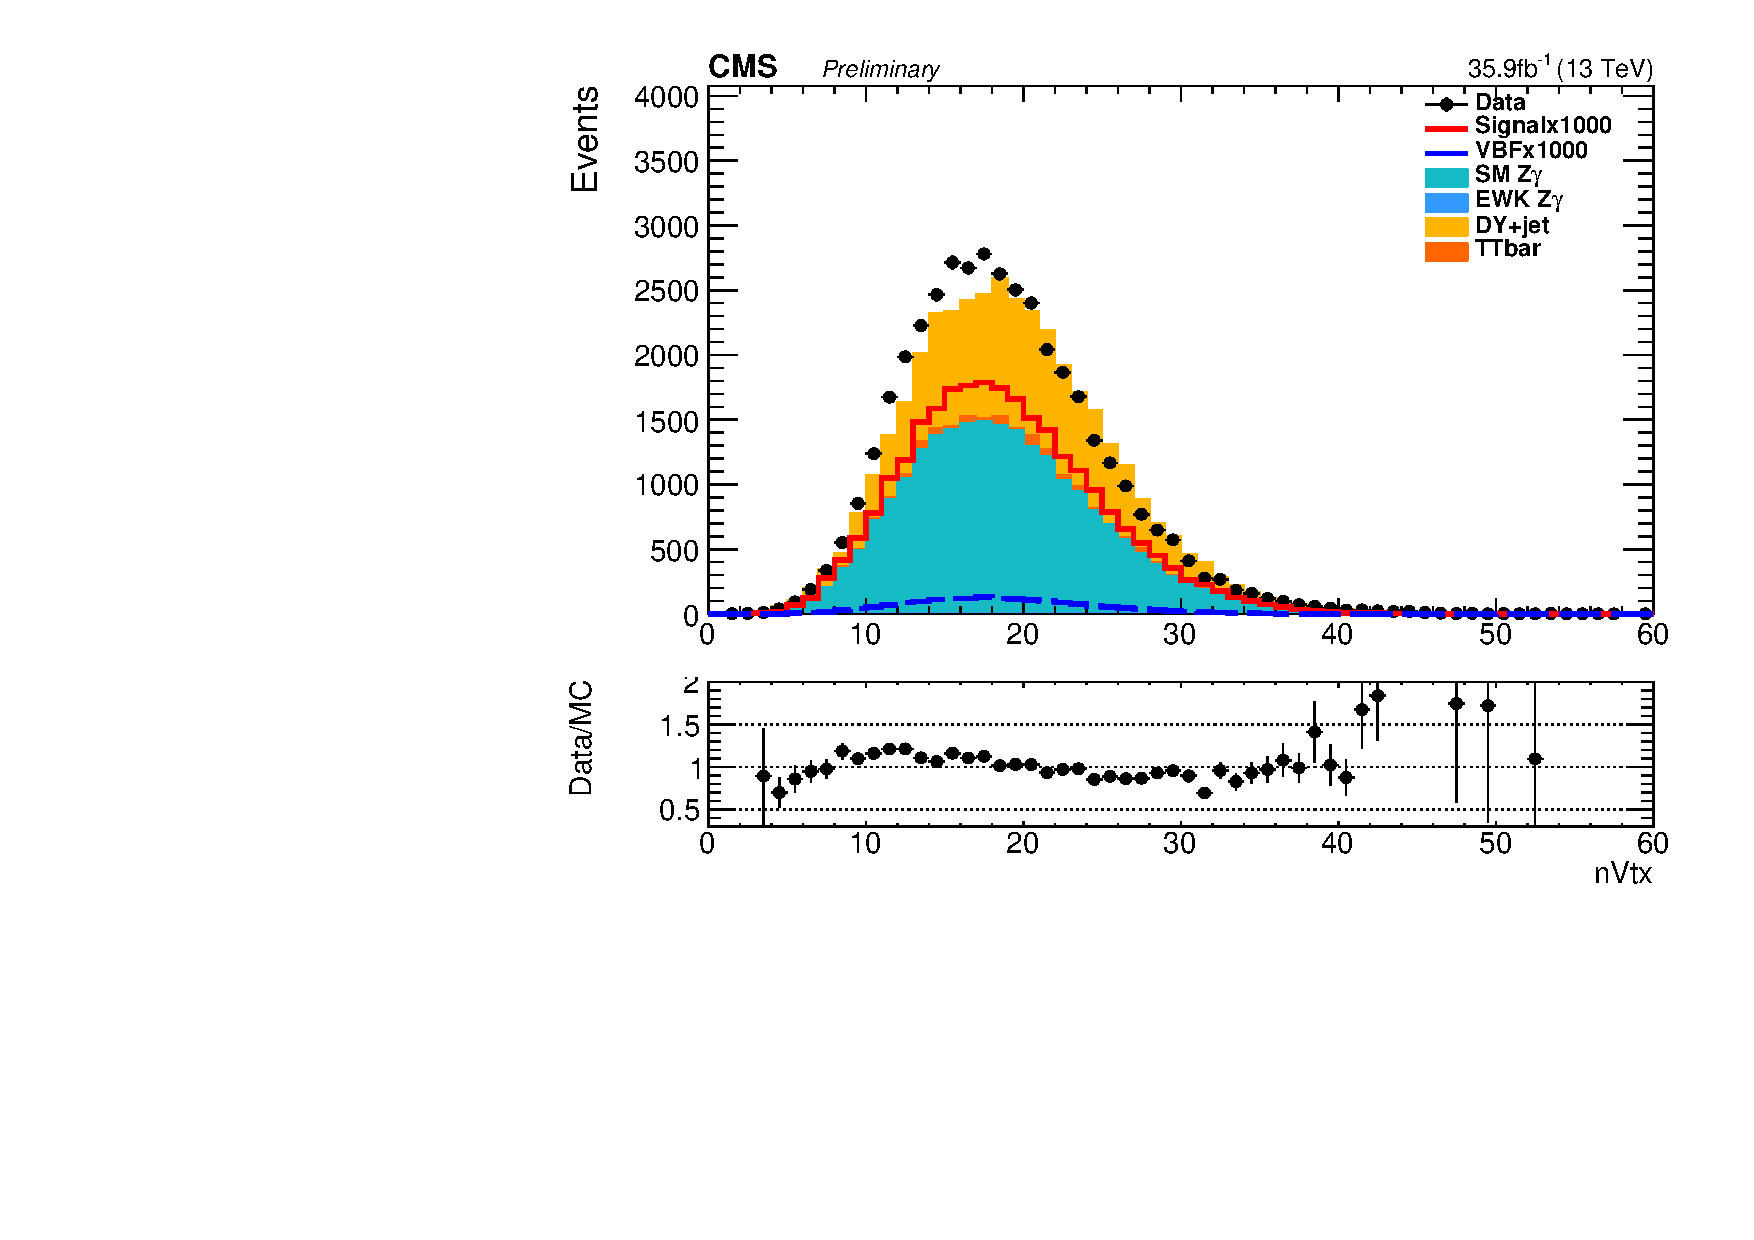
\includegraphics[width=0.3\textwidth]{fig/pileup/ele_kin_nVtx_valid_Legacy16_HLT.pdf}
     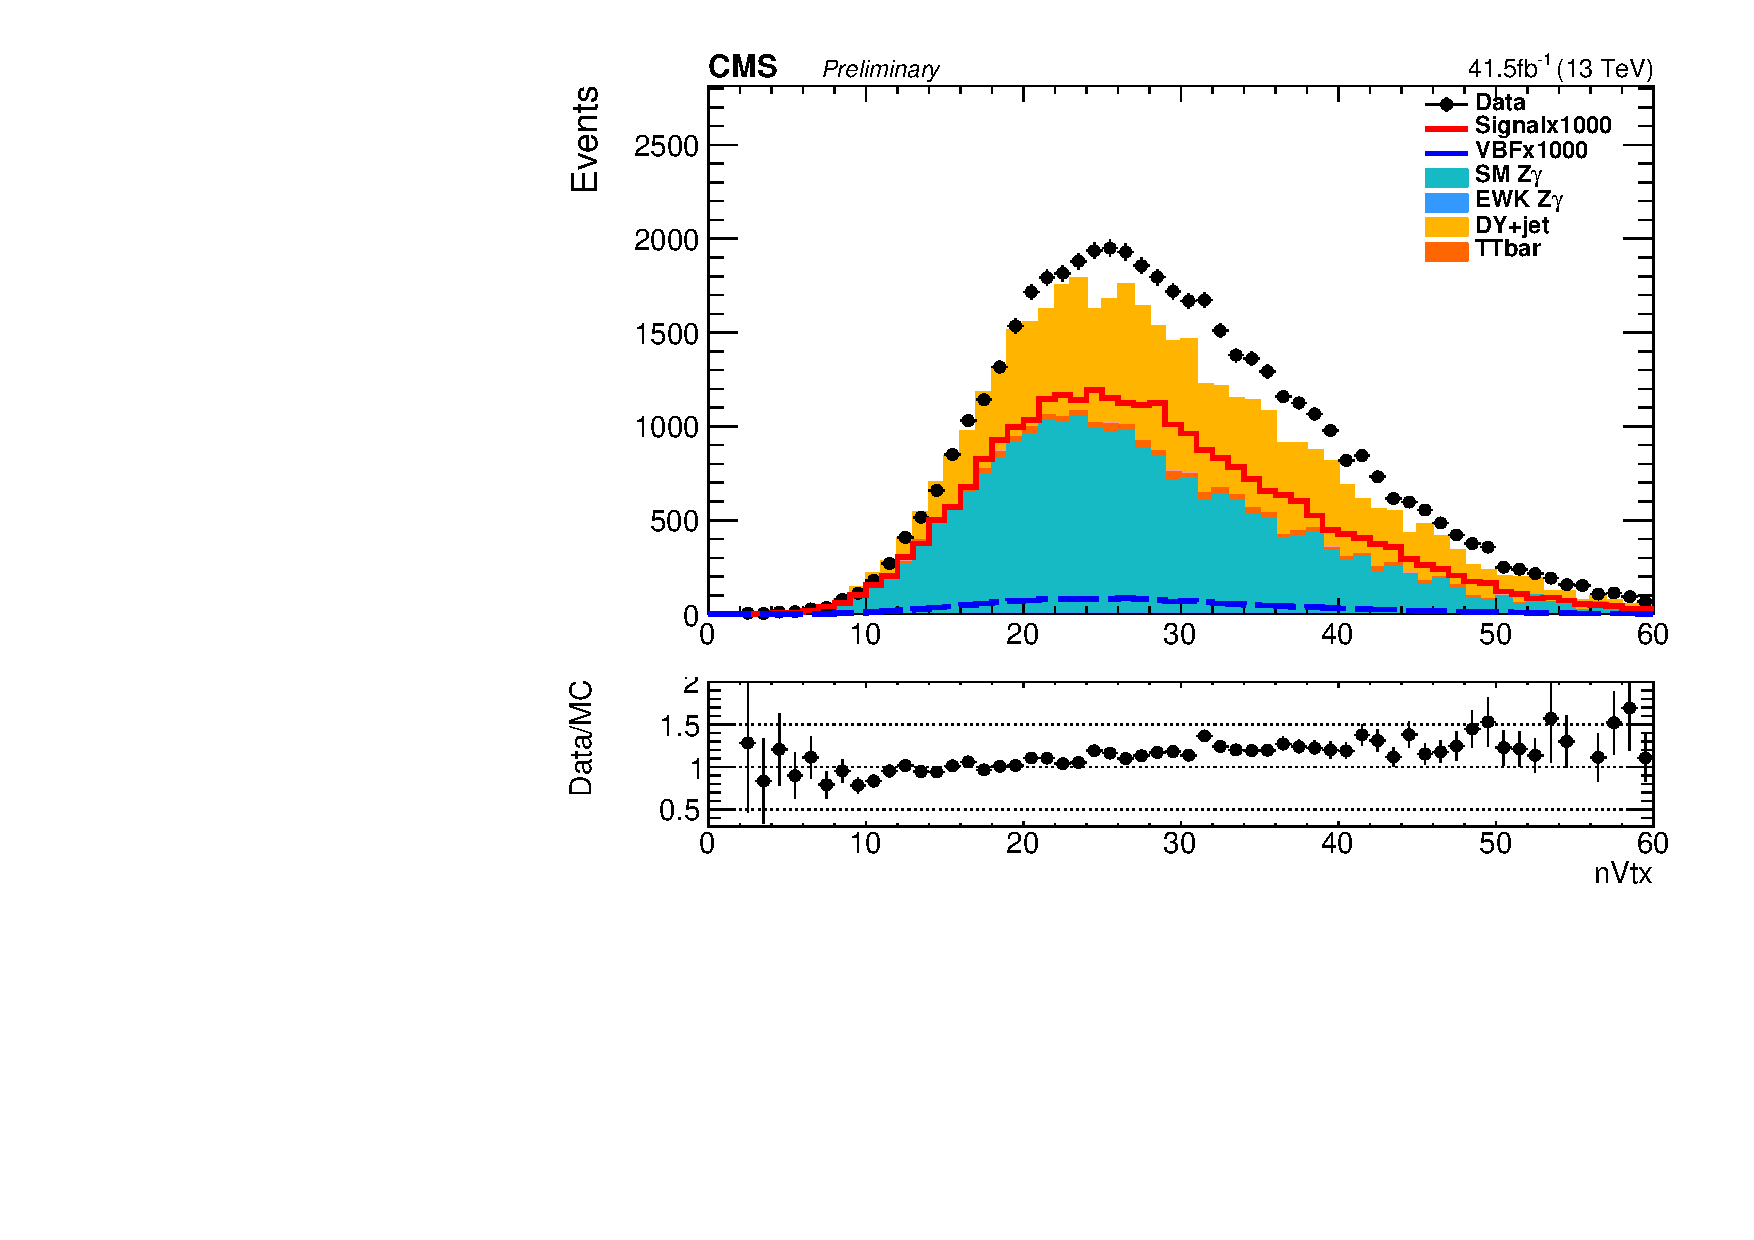
\includegraphics[width=0.3\textwidth]{fig/pileup/ele_kin_nVtx_valid_Rereco17_HLT.pdf}
     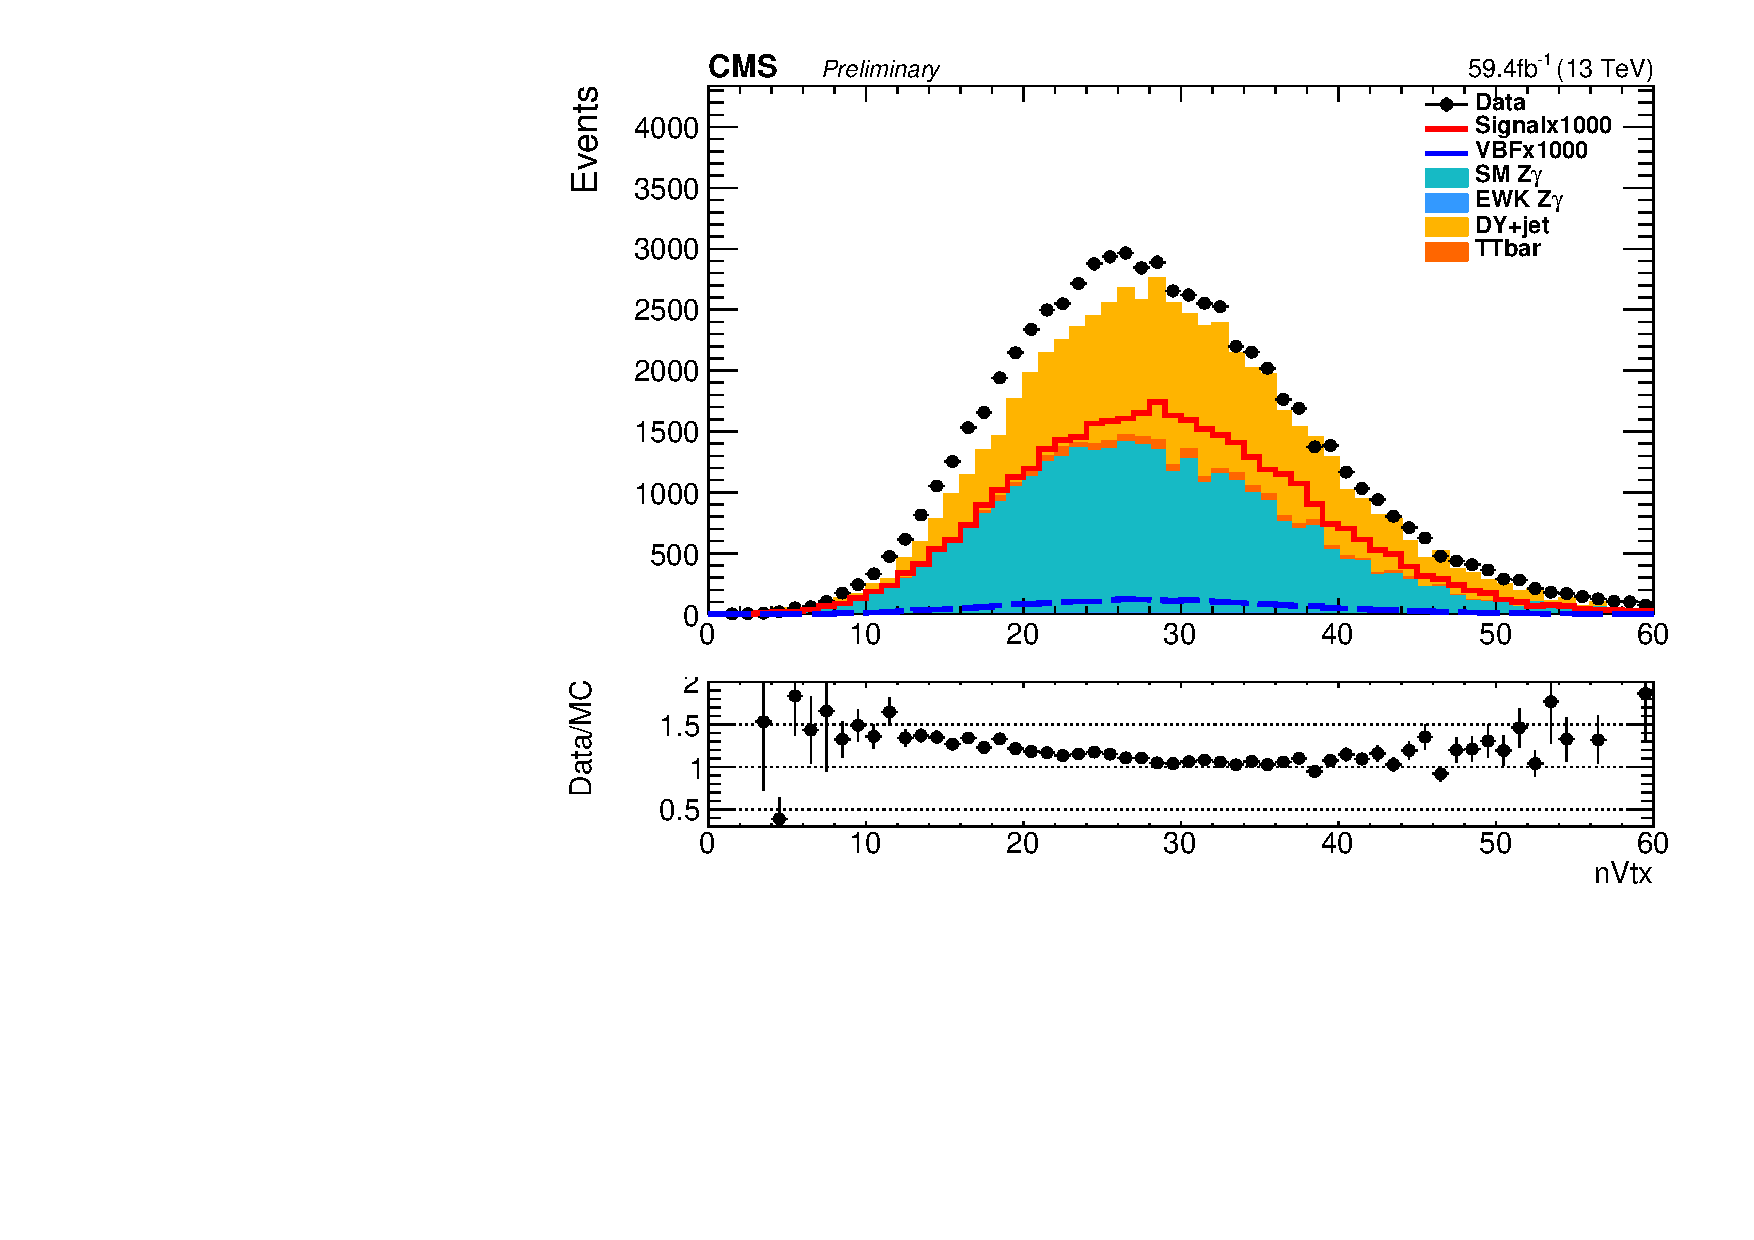
\includegraphics[width=0.3\textwidth]{fig/pileup/ele_kin_nVtx_valid_Rereco18_HLT.pdf}
  \end{center}
\caption{Distribution of the number of primary vertices in data and simulation shown for the electron channel after 2 leptons and 1 photon are selected. Left to right: 2016, 2017, 2018. The pileup cross section is taken to be 66 mb, 72.4 mb, and 80 mb for 2016, 2017, and 2018 respectively.}
\label{fig:puwei}
\end{figure}

\section{L1 Prefiring Problem}\label{sec:L1}
In 2016 and 2017, a gradual timing shift of the ECAL was not properly propagated to 
L1 trigger primitives (TP) resulting in a significant fraction of high eta TP 
being mistakenly associated to the previous bunch crossing. 
Since Level 1 rules forbid two consecutive bunch crossings to fire, 
an unpleasant consequence of this (in addition to not finding the TP in the bx 0) 
is that events can self veto if a significant amount of ECAL energy is found in the region 
of $2.<|\eta|<3$. This effect is not described by the simulations \cite{L1_prefire}.\\

The JETMET twiki provides a recipe to compute the probability for an event not to prefire, that can then be applied to the simulations. This is achieved with an EDProducer that runs over all offline photons and jets found in the event and assign them a prefiring probability. 

The final event weight is obtained as the product of the non prefiring probability of all objects (measured using unprefirable events), namely:
\begin{equation}
	\omega = 1 - P(Prefiring) = \prod_{i=photon,jets}(1-\epsilon_i^{pref}(\eta,\pt^{EM}))
\end{equation}

The impact of the L1 prefiring for electrons (muons) is a 1.4 (0.8)\% 
loss in signal yield for 2016 and 2.4 (1.1)\% 
loss in signal yield for 2017.

